\chapter{مقدمه}\label{Chap:Chap1}
\minitoc

\section{تعریف مسئله} \label{chap1:prob_define}

\subsection{‌مسئله گفتگو}
خلق ماشینی که بتواند با انسان از طریق زبان طبیعی به گفتگو بپردازد، یکی از آرزو‌های اولیه و در عین حال از اهداف نهایی و غایی هوش مصنوعی می‌باشد.
این ماشین بایستی بتواند ویژگی‌های گفتگوی انسانی را به خوبی تقلید کند و همچنین قادر باشد که در طیف موضوعی وسیعی که می‌تواند از راجع به تئوری نسبیت انیشتین تا آخرین اخبار اقتصادی روز گسترده ‌شده باشد صحبت کند.
همچنین این ماشین هوشمند می‌تواند این امتیاز اضافه را نیز داشته باشد که از طریق گفتگو با انسان قادر به فهمیدن وظایف مختلف اطلاعاتی (برای مثال رزرو یک فیلم در یک سینما) و انجام آن ها برای انسان باشد.
نیل به این هدف در نهایت می‌تواند موجب پیدایش سامانه‌های هوشمندی نظیر
\trans{دستیار مجازی}{Virtual Assistant}
، 
\trans{سامانه توصیه‌گر}{Recommender System}
 و 
\trans{روبات گپ‌زن}{Chatbot}
  شود که همگی از طریق 
بستر زبان طبیعی، سعی در ارتباط با عامل انسانی پیش‌ روی خود دارند.

برای نزدیک شدن به این مهم، ماشین‌ها بایستی بتوانند تعدادی توانایی کلیدی را کسب کنند. از جمله این توانایی ها می‌توان به درک زبان طبیعی، به کار بستن حافظه برای حفظ و به یادآوری مفاهیم و دانش در قالب زبان طبیعی،‌ استنتاج در مورد مفاهیم و در نهایت توانایی تولید پاسخ مناسب (چه از نظر صحت زبانی و چه از نظر ارتباط با محتوای گفتگو) اشاره کرد.

با وجود پیشرفت‌های گسترده و چشم‌گیر هوش مصنوعی در سالیان اخیر و ظهور و تکامل  و یادگیری ژرف اما تلاش‌ها برای خلق یک سیستم مکالمه‌گر با ویژگی‌های مذکور تا به امروز ناکام مانده‌اند و این مساله یک مساله باز و حل نشده باقی مانده است.
وظیفه مکالمه را در واقع می‌توان به نوعی محل تلاقی سه حوزه تحقیقاتی
هوش مصنوعی، پردازش زبان و بازیابی اطلاعات دانست.
هم اکنون توجه زیادی از سمت محققین این سه حوزه به مسئله مکالمه معطوف شده است و هر پیشرفتی در روند این مساله می‌تواند بیانگر پیشرفتی عظیم در این سه حوزه باشد.

علاوه بر مطالب بالا می‌توان به طور مخصوص از زاویه دید حوزه پردازش زبان نیز وظیفه مکالمه را بررسی کرد. عمده وظایف موجود در حوزه پردازش زبان طبیعی را می‌توان در دو دسته فهم و درک زبان طبیعی و تولید زبان طبیعی گروه‌بندی کرد. اهمیت وظیفه مکالمه در حوزه پردازش طبیعی در این است که تحقق آن در واقع نشان از تحقق در هر دو حوزه فهم زبان طبیعی و تولید زبان طبیعی دارد و در نتیجه وظیفه مکالمه را می‌توان به نوعی مادر تمام وظایف پردازش زبان در نظر گرفت. یکی از اهمیت‌های این موضوع می‌تواند این باشد که همان‌گونه که امروزه مدل‌های 
\trans{از پیش آموزش داده شده}{pretrained}
 با استفاده از مقدار زیادی داده روی وظیفه مدل زبانی آموزش می‌بینند و سپس با کمک 
\trans{انتقال یادگیری}{Transfer Learning}
  روی وظایف دیگری تنظیم می‌شوند، شاید بتوان در آینده همین رویکرد را به جای استفاده از مدل‌های زبانی با مدل‌های مخصوص مکالمه دنبال کرد.




\subsection{‌انواع مسائل گفتگو}

سامانه‌های مکالمه را از منظر مسئله‌ ی مورد هدف گذاری شده‌شان می‌توان به سه دسته تقسیم کرد. این سه دسته مسئله پرسش و پاسخ، تکمیل وظیفه و گپ‌زنی 
هستند.

در مساله پرسش و پاسخ، معمولا با سه عنصر کاربر انسانی، عامل هوشمند و یک منبع دانش مواجه هستیم. منبع دانش در واقع می‌تواند یا به صورت مجموعه‌ای از داده‌های بدون ساختار مانند اسناد متنی یا به صورت یک پایگاه دانش ساختار یافته مانند گراف دانش باشد. روند این مساله به این صورت است که کاربر انسانی یک پرسش را در بستر زبان طبیعی مطرح می‌کند و عامل هوشمند بایستی بتواند با توجه به سوال، مفاهیم مربوط را از پایگاه دانش استخراج کرده و گاها روی آن‌ها عملیات استنتاج انجام دهد. پس از استخراج و استنتاج این مفاهیم سپس عامل هوشمند بایستی پاسخ مربوط را در بستر زبان طبیعی تولید کرده و به کاربر انسانی انتقال دهد.
عامل‌های هوشمند مخصوص مسائل پرسش و پاسخ معمولا فاقد حافظه برای مکالمه هستند و هر دور مکالمه آن‌ها با کاربر معمولا تنها یک رفت و برگشت طول می‌کشد. با توجه به کاربرد‌های گسترده علمی و صنعتی که عامل‌های هوشمند پرسش و پاسخ می‌توانند داشته باشند، از سال های قبل توجه و انرژی بسیاری از محققین روی این مساله جذب شده است و اکنون تعداد زیادی دادگان برای مسائل با تنظیمات گوناگون پرسش و پاسخ طراحی و جمع‌آوری شده اند. از مشهورترین این دادگان می‌توان به دادگان 
\lr{SQUAD}
، پرسش‌های طبیعی و 
\lr{CNN}
  و 
\lr{Wiki QA}
   اشاره کرد
\cite{squad_paper, cnnqa_paper, naturalqa_paper, wikiqa_paper}.



در مقابل، دسته بعدی سامانه‌های مکالمه‌گر،‌ مکالمه‌گر‌های 
\trans{وظیفه محور}{Task Oriented}
 هستند که در پی این هستند تا با استفاده از زبان طبیعی یک ارتباط موثر بین خود و عامل انسانی فراهم کنند. این ارتباط در نهایت موجب بهبود درک متقابل میان این دو شده و موجب می‌شود تا وظیفه تعیین شده
برای این سامانه به خوبی انجام شود.
این وظیفه می‌تواند برای مثال رزرو بلیت سینما، تنظیم کردن یاد‌آور زمانی،‌خرید از فروشگاه اینترنتی یا انواع وظایف دیگر باشد.
این سامانه‌ها به علت کاربرد صنعتی، گسترش بیشتری از دسته سامانه‌های گپ‌زن داشته‌اند و در نتیجه امروزه نمونه‌های زیادی از آن‌‌ها را، همچون دستیارهای مجازی هوشمند ارائه شده توسط شرکت‌هایی نظیر گوگل، اپل	 و آمازون و ... می‌توان مشاهده کرد. معماری و روش استفاده شده در این دسته سامانه‌ها بیشتر به شکل استفاده از معماری 
\trans{پیمانه‌ای}{Modular}
است. 
برای درک بهتر معماری پیمانه‌ای این سامانه‌ها شکل 
\ref{fig:chap1s:modular}
آورده شده است.
همچنین این سامانه‌ها عمدتا برای مشخص‌کردن ساختار وظیفه معینشان، از 
\trans{هستی شناسی}{Ontology}
 های تهیه شده توسط افراد خبره استفاده می‌کنند.
نکته مهمی که در خصوص این دسته‌ سامانه‌ها می‌توان متذکر شد این است که با وجود توسعه و رشد چشمگیر آن‌ها، از زبان صرفا به عنوان یک ابزار برای رد و بدل کردن اطلاعات استفاده می‌کنند و به عبارتی بهتر زبان بیش‌تر از آن‌ که برای آن‌ها نقش هدف را داشته باشد، نقش ابزاری برای نیل به وظایف آن‌ها را دارد. این مطلب را می‌توان از معیارهای ارزیابی مطرح شده برای آن‌ها نیز برداشت کرد؛ به این صورت که اکثر آن‌ها با کیفیت بودن یک سامانه مکالمه وظیفه محور را معادل با درست و البته زود انجام شدن مکالمه با کاربر می‌دانند و توجهی به میزان سرگرم‌کردن و مشتاق‌کردن کاربر به ادامه دادن مکالمه در هنگام گفتگو ندارند، حال آن که این حقیقت در مورد دسته‌ سامانه‌های مکالمه گپ‌زن همانطور که در ادامه خواهیم دید، کاملا برعکس است.

\begin{figure}[h]
	\centering
	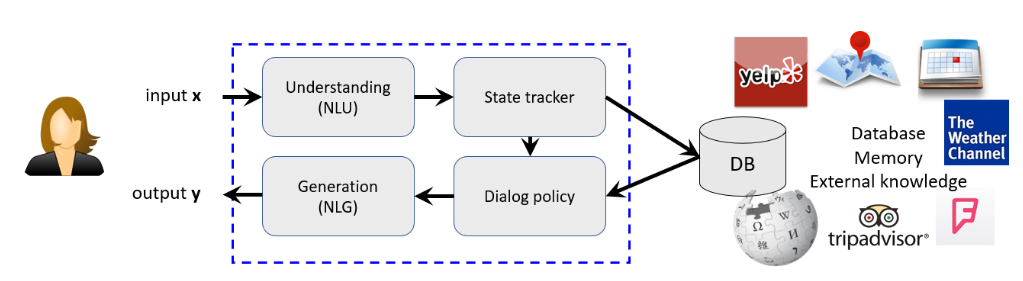
\includegraphics[width=1\textwidth]{images/chap1/modular.png}
	\caption{
		نمایی از معماری‌ پیمانه‌ای سامانه‌های مکالمه وظیفه محور
		\cite{Gao_Neural_Approaches}
	}
	\label{fig:chap1s:modular}
\end{figure}


در طرف مقابل اما، سامانه‌های مکالمه گپ‌زن قرار دارند که هدف آن‌ها یادگیری و تقلید و اجرای گفتگوی انسانی و به طور عمومی گفتگو در یک
\trans{دامنه باز}{Open Domain}
است.
این دسته از سامانه‌های مکالمه، زودتر از سامانه‌های مکالمه وظیفه محور پا به عرصه گذاشتند.
از نمونه‌های اولیه این مکالمه‌گر‌ها می‌توان به الیزا و پری اشاره کرد
\cite{weizenbaum1966eliza, parry}
.
اما در ادامه از طرفی با کمبود دادگان مناسب برای این دسته از سامانه‌ها و از طرفی تمرکز صنعت و پژوهشگران حوزه‌های مختلف بر روی سامانه‌های مکالمه‌گر وظیفه محور، روند توسعه و پیشرفت گپ‌زن‌ها دچار توقف و رکودی طولانی شد. تا این که در سالیان اخیر به لطف پیشرفت یادگیری ژرف و البته فراهم‌ شدن دادگان مناسب برای آموزش این مکالمه‌گر‌ها، روند پژوهش و توسعه این سامانه‌های گپ‌زن دوباره شتاب نویی به خود گرفت.

یکی از تفاوت‌های اساسی سامانه‌های مکالمه‌گر گپ‌زن با سامانه‌های مکالمه‌گر وظیفه محور در این است که گپ‌زن‌ها بدون نیاز به دانش تخصصی (نظیر آن چه که در وظیفه محور ها مطرح شد) می‌توانند تنها از روی دادگان و با یک شبکه عصبی به صورت
\trans{انتها به انتها}{End to End}
آموزش ببینند. از این رو گاها به این سامانه‌ها، سامانه‌های مکالمه 
\trans{داده محور}{Data Driven}
 نیز گفته می‌شود.

	
\subsection{انواع اصطلاحات علمی در رابطه با سامانه مکالمه‌گر}

در این جا لازم است تا قبل از پرداختن به موضوعات بعدی، یک ابهام احتمالی برطرف شود. در صورت جستجو درباره سامانه‌های مکالمه در مقالات علمی با اصطلاحات و ادبیات علمی گوناگونی جهت نام بردن سامانه‌های مکالمه مواجه می‌شویم. از اصطلاحات پرتکرار می‌توان لغات 
\lr{Dialouge System, Conversational AI, Chatbot}
و
\lr{Chitchat}
را نام برد.
با این که قرارداد یا استاندارد مشخصی برای منظور این واژه‌ها وجود ندارد اما با جستجو در مقالات منتشر شده می‌توان پی‌برد که هر کدام از این اصطلاحات با دیگری تفاوت  معنایی اندکی دارند. اصطلاح 
\lr{Dialouge System}
در کل به صورت عام به سامانه‌های مکالمه‌گر وظیفه‌محور و گپ‌زن اشاره می‌کند. 
اما اصطلاحات 
\lr{Conversational AI}
و
\lr{Conversation Model}
که در سال‌های اخیر و آغاز دوباره اوج‌گیری سامانه‌های داده محور مورد استفاده قرار گرفته‌اند، به مدل سازی مکالمه با استفاده از یادگیری ماشین و شبکه‌های عصبی اشاره می‌کنند و بیشتر برای سامانه‌های مکالمه گپ‌زن به کار می‌روند (به نوعی این اصطلاح می‌خواهد بین سامانه‌های مکالمه قدیمی که 
\trans{مبتنی بر قانون}{Rule-Based}
بود‌ه‌اند و سامانه‌های جدید که مبتنی بر شبکه عصبی هستند تمایز را نشان دهد).
اصطلاحات 
\lr{Chitchat} 
و 
\lr{ChatBot}
نیز به طور خاص به سامانه‌های مکالمه گپ‌زن اشاره دارند و در پی تمایز آن ها از سامانه‌های مکالمه وظیفه‌محور هستند. 
در این پژوهش نیز ما غالبا از اصطلاحات گپ‌زن  و سامانه مکالمه برای اشاره به سامانه‌های مکالمه گپ‌زن و داده محور استفاده می‌کنیم و به ندرت به سامانه‌های مکالمه وظیفه محور اشاره می‌کنیم. 

\subsection{مساله گپ‌زن دانش بنیان}\label{chap1:knowledge_problem}
در سال‌های اخیر پس از موفقیت‌های یادگیری ژرف  و مدل‌های متفاوت آن در وظیفه ترجمه ماشینی و همچنین شباهت نسبی این وظیفه به وظیفه گپ‌زن‌ها، پژوهشگران عرصه سامانه‌های مکالمه‌گر نیز به فکر استفاده از مدل‌های ترجمه ماشینی جهت حل وظیفه مکالمه افتادند. این تلاش اکنون به صورت خاصی در استفاده از مدل‌های دنباله به دنباله (که خود برخاسته از مساله ترجمه ماشینی هستند) تجلی پیدا کرده است. پس از استفاده از مدل‌های دنباله به دنباله در مسئله گپ‌زن‌ها با این که در ابتدا رشد و پیشرفتی شگرف و نتایجی چشمگیر در این مسئله مشاهده شد
؛
اما آرام آرام چالش‌ها جدیدی پیش روی محققین این حوزه پدیدار شدند
\cite{a_neural_conv_model}.
 این چالش‌ها به عقیده برخی محققین، به علت پیچیده‌تر بودن مسئله گفتگو نسبت به ترجمه ماشینی و استفاده صرف و بدون ارتقا مدل‌های ترجمه ماشینی برای این مساله پیچیده‌تر بوده است. از جمله این چالش‌های اساسی می‌توان به 
\trans{کسل کننده بودن پاسخ}{Response Blandness}
ها، عدم
\trans{ثبات مکالمه‌گر}{Speaker Consistency}
 و البته 
\trans{دانش‌بنیان}{Knowledge Grounded}
نبودن گپ‌زن ها اشاره کرد.

گپ‌زن‌های امروزی علی رغم توانایی در فهم زبانی و همچنین تولید پاسخ با صحت دستور زبانی اما همچنان قادر به 
گفتگو در دامنه‌های مختلف و تولید پاسخ با ارزش اطلاعاتی نمی‌باشند. در واقع گپ‌زن‌های امروزی با این که گفتگوی رد و بدل شده در بستر زبان را به خوبی می‌فهمند اما در به کارگیری حافظه و همچنین دانش بیرونی دچار ضعف اساسی هستند که این ضعف لطمه شدیدی به غایت آن‌ها یعنی توانایی گفتگو در دامنه باز وارد می‌کند. در واقع همانطور که در ابتدا گفته شد، یک گپ‌زن دامنه باز باید قادر به فهم مفاهیم زبانی باشد، مکانیزمی را برای نگهداری و استفاده از یک حافظه پیاده‌سازی کند، قادر به استخراج و فراخوانی دانش مرتبط با گفتگو باشد، مفاهیم استخراج‌ شده را با یکدیگر ترکیب کرده و از آن‌ها استنتاج انجام دهد و در نهایت پاسخی مناسب تولید کند
\cite{wizard}
.
حال آن که در صورت استفاده صرف از مدل های دنباله به دنباله بدون به کارگیری هیچ دانش خارجی، گپ‌زن شبیه به کودکی می‌شود که قادر به فهمیدن و صحبت‌کردن هست اما به علت نداشتن دانش خارجی، قادر به صحیح و کامل پاسخ دادن نمی‌باشد.

یک گپ‌زن دامنه‌باز دانش بنیان بایستی بتواند موجودیت‌ها و موضوعات مطرح شده در گفتگو را تشخیص دهد؛ آن‌ها را با حقایق جهان واقعی مرتبط سازد و سپس سایر اطلاعات 
پیش زمینه مرتبط با آن‌ها را از پایگاه دانش خود استخراج نماید. 
در این صورت است که می‌تواند در گام بعدی پاسخی را برای عامل انسانی فراهم کند که خود دارای ارزش اطلاعاتی در مورد موجودیت‌های مطرح شده در گفتگو است. 
تفاوت مدل‌های فعلی مطرح شده دانش بنیان در نوع نگاه به راه‌حل مراحل مذکور 
از جمله نوع پایگاه دانش مورد استفاده، نحوه عملکرد و معماری مدل دخیل کردن تاریخچه و نحوه غملکرد و معماری مدل زایشگر پاسخ
است: از این رو می‌توان این راه‌حل ها را با توجه به این اختلاف سلیفه مورد بررسی و مقایسه قرار داد. 

\section{اهمیت تحقق گپ‌زن دانش بنیان} \label{chap1:knowledge_importance}

اهمیت دستیابی به دانش بنیان کردن گپ‌زن ها را از دو زاویه می‌توان تحلیل کرد. اولا اضافه کردن دانش به گپ‌زن و استفاده از آن باعث می‌شود تا به جای پاسخ‌های احتمالی بی محتوا، پاسخ‌های محتوامند و دارای ارزش اطلاعاتی تولید شوند که خود می‌تواند باعث افزایش جذابیت گپ‌زن برای کاربر انسانی شود. به علاوه گپ‌زن دانش بنیان را می‌توان در کاربردهای متنوعی با صرفا تعویض منبع دانش آن استفاده کرد. در نتیجه از گپ‌زن به عنوان یک سامانه توصیه‌گر در کاربردهای مختلف 
می‌توان بهره برد. یکی از دیگر مزایای دانش بنیان بودن گپ‌زن می‌تواند این باشد که می‌توان منبع دانش متصل به گپ‌زن را در هر ثانیه به روز رسانی کرد و مطمئن بود که گپ‌زن در هر لحظه نسبت به آخرین رخدادها و تغییرات و حقایق جهان خارجی آگاه است و می‌تواند درباره آن‌ها بحث و گفتگو کرده و اطلاعاتی را به کاربر انتقال دهد.

اما از سوی دیگر مسئله گپ‌زن دانش بنیان را می‌توان به شکل مکالمه شرطی نیز در نظر گرفت. با ارائه یک مدل قابل تعمیم برای شرطی سازی گفتگو مبتنی بر دانش، این احتمال وجود دارد که برای دیگر مسائل مکالمه شرطی نظیر دخیل کردن شخصیت یا احساسات در گپ‌زن نیز بتوانیم مدلی مناسب ارائه دهیم.

به طور  کلی از منظر کاربرد عملیاتی و صنعتی نیز می‌توان از گپ‌زن دانش بنیان در کاربرد‌هایی نظیر سامانه‌های توصیه‌گر،
 جایگزین کردن اپراتور‌های انسانی پاسخگو با اپراتور‌های هوشمند، دادن مشاوره تخصصی به کاربران نظیر مشاوره پزشکی، ارائه خدمات محتوامحور نظیر پیشخوان سایت‌های خبری و البته آموزش الکترونیکی بهره برد.  

\section{مدل‌های پایه گفتگو} \label{chap1:history}

\subsection{ایده‌پردازی اولیه از روی مسئله ترجمه ماشینی}

در ادامه در این بخش، مدل‌های  عصبی پایه برای حل مسئله گفتگو مورد بررسی و بحث قرار می‌گیرند. این بررسی و بحث در فهم بهتر مسیر تکامل مدل‌های گفتگو و چالش‌هایی که این مدل‌ها در طی این مسیر با آن‌ها مواجه شده اند (از جمله چالش دانش‌ بنیان نبودن) مفید واقع خواهند شد و درک بهتری از وضعیت مساله و ایده‌های ممکن برای حل آن حاصل خواهد کرد.

اولین روش‌های حل مساله گپ‌زنی با آموزش انتها به انتها 	از روی دادگان مکالمه، از روش‌های آماری حل مسئله ترجمه ماشینی الهام گرفتند و در ادامه به تبع آن رویکرد و معماری 
\trans{رمزگذار}{Encoder}
و
\trans{رمزگشا}{Decoder}
متعلق به ساختار دنباله به دنباله آن را نیز سرلوحه خود قرار دادند. ایده کلی مدل‌ کردن مسئله گپ‌زنی به ترجمه ماشینی به این صورت است که تاریخچه گفتگو به عنوان جمله زبان مبدا و پاسخ گفتگو نیز به عنوان جمله زبان مقصد در نظر گرفته شوند و با استفاده از مدل‌های موجود برای ترجمه ماشینی بتوان تابع تبدیل تاریخچه گفتگو به پاسخ مطلوب را مدل کرد
\cite{ritter-etal-2011-data}
.
اولین تلاش جدی در این زمینه را می‌‌توان تلاش سردونی در ۲۰۱۵ دانست که یک مدل بر پایه 
\trans{شبکه عصبی بازگشتی}{Recurrent Neural Network}
را برای تولید پاسخ مکالمه پیشنهاد داد و همچنین توانست از تاریخچه گفتگو در مدل خود استفاده کند
\cite{DBLP:journals/corr/SordoniGABJMNGD15}
.
با وجود این که ظاهرا به نظر می‌رسد که مسئله ترجمه ماشینی و مکالمه به یکدیگر شباهت زیادی دارند، اما استفاده از مدل‌های ترجمه ماشینی راه حل بی عیب و نقصی برای مساله مکالمه محسوب نمی‌شوند و در عمل این مدل‌ها با ایرادات واضح و آشکاری مواجه هستند. این ایرادات می‌توانند برآمده از ذات متفاوت مسائل ترجمه و مکالمه باشند. در ادامه تعدادی از این ایرادات 
مورد بررسی و بحث قرار می‌گیرند و همچنین تعدادی از راهکارهای پیشنهادشده برای حل این چالش‌ها نیز مورد اشاره واقع خواهند شد. 


یکی از چالش‌های موجود در مسئله مکالمه طولانی بودن تاریخچه مکالمه است. پس از موفقیت شبکه LSTM در حل معضل 
\trans{گرادیان میرا}{Vanishing Gradient}
و 
\trans{گرادیان در حال انفجار}{Exploding Gradient}
در مسئله ترجمه ماشینی این مدل در ادامه در مسئله مکالمه مورد استفاده قرار گرفت و توانست عملکرد مثبتی را نسبت به روش‌های موجود از خود نشان دهد
\cite{A_Neural_Conversational_Model}.

از آنجایی که نشان داده شده است که LSTM قادر به رمزکردن موثر متونی با حداکثر طول ۵۰۰ کلمه است
\cite{DBLP:journals/corr/abs-1805-04623}
؛
تلاش‌هایی در جهت ارائه مدل‌هایی با توانایی به یادسپاری بیشتری صورت گرفت که در نهایت این تلاش‌ها منجر به طراحی مدل‌های بازگشتی سلسله مراتبی برای مسئله مکالمه شد
\cite{DBLP:journals/corr/SerbanSBCP15, DBLP:journals/corr/XingWWZHM17, DBLP:journals/corr/SordoniBVLSN15}.
برای درک بهتر می‌توان یکی از این مدل‌ها را در نظر گرفت که از دو سطح بازگشتی تشکیل شده است که با یکدیگر ترکیب شده اند
\cite{DBLP:journals/corr/SordoniBVLSN15}.
شبکه بازگشتی بیرونی گفتگو را به شکل دنباله‌ای از نوبت‌های دو شخص گفتگوکننده می‌بیند و شبکه بازگشتی داخلی نیز هر نوبت از این مکالمه را به صورت دنباله‌ای از کلمات می‌بیند. مزیت این مدل در این است که اجازه می‌دهد محتوای یک نوبت از گفتگو راحت تر در نوبت‌های بعدی گفتگو منتشر شود و همچنین مشکل گرادیان میرا در طول شبکه خفیف شود
\cite{Gao_Neural_Approaches}.

پس از ابداع مکانیزم
\trans{توجه}{Attention}
در شبکه‌های رمزگذار و رمزگشا برای وظیفه ترجمه ماشینی و بهبود معیار‌های این وظیفه، اما بر خلاف انتظار، استفاده از این مکانیزم در وظیفه گفتگو نتوانست به قدر توقع باعث بهبود مدل‌های مکالمه شود. این پدیده می‌تواند به این صورت توضیح داده‌ شود که مکانیزم توجه به صورت موثری سعی در تراز کردن کلمات جمله مبدا و مقصد مدل دارد. این سعی با این که در مسئله ترجمه ماشینی به علت حضور کلمه مبدا با محتوای مشابه و جفت در طرف جمله مقصد مفید واقع می‌شود اما در مسئله گپ‌زنی گاها به این علت که محدوده جمله پرسش ممکن است به هیچ کلمه‌ای در جمله پاسخ نگاشت نشود ناکام می‌ماند
\cite{Gao_Neural_Approaches}.
در واقع این رخداد این مطلب را به ما یادآوری می‌کند که ذات مساله گفتگو با مساله ترجمه ماشینی متفاوت بوده و حل آن نیازمند به ساختارهای متفاوت‌تری است.

\subsection{چالش‌های پیش روی سامانه‌های مکالمه}
مدل‌های کنونی گپ‌زنی اکنون با مشکلات و چالش‌هایی مواجه هستند که اکثر این چالش‌ها برآمده از طبیعت و ذات مکالمه و خاص این مسئله هستند. اکثر پژوهش‌ها و تلاش‌های اخیر در حوزه مکالمه‌گرها در پی رفع و یا تخفیف این مشکلات هستند. در ادامه تعدای از این مشکلات 
به صورت اجمالی مورد توضیح واقع شده و در نهایت ارتباط آن‌ها با مسئله هدف‌گرفته‌شده یعنی دانش بنیان کردن گپ‌زن ها تصویر خواهد شد.

یکی از مشکلات رایج در بین گپ‌زن‌هایی با معماری دنباله به دنباله تمایل آن‌ها به تولید پاسخ‌هایی واضح و دارای بار معنایی کم یا در حالت  خفیف‌تر عدم تنوع در پاسخ‌های تولیدی است. این پاسخ‌ها اغلب جملاتی مانند 
"نمی‌دانم" و یا "باشه" هستند که در دادگان آموزشی مورد استفاده توسط گپ‌زن، دارای میزان فراوانی بالایی می‌باشند.

یکی دیگر از مشکلات موجود در گپ‌زن‌ها عدم ثبات شخصیت گپ‌زن است. برای درک بهتر می‌توان مثالی را در نظر گرفت که در آن گپ‌زن در جواب به پرسش "چه کاره هستی؟" پاسخ "من یک پزشک هستم" و در پاسخ به پرسش "تو چه شغلی داری؟" پاسخ "من یک نجار هستم" را تولید کند. این مشکلات اغلب در پاسخ به سوالاتی هویدا می‌شوند که آن پاسخ در دادگان آموزشی گپ‌زن دارای چندین پاسخ متنوع بوده است.

حدس اولیه ما در این جا این است که هر دو مشکل کسل کننده پاسخ‌ها و عدم ثبات شخصیت گپ‌زن از معماری دنباله به دنباله ریشه می‌گیرند. معماری دنباله به دنباله اولین بار برای مساله ترجمه ماشینی مطرح شد و نتایج قابل قبولی نیز در این مساله به دست آورد
\cite{seq2seq_paper}.
در مساله ترجمه ماشینی ما با پدیده یک به یک بودن رشته‌های ورودی و خروجی مواجه هستیم. به این معنی که اغلب جملات زبان مبدا به یک جمله در زبان مقصد نگاشت می‌شوند و اغلب جملات زبان مقصد هم به یک جمله در زبان مبدا نگاشت می‌شوند. اما در مساله مکالمه ما نه تنها با قالب یک به یک رشته‌های مبدا و مقصد مواجه نیستیم که با یک حالت چند به چند روبرو هستیم. به این معنی که برخی پرسش‌ها مانند "چه کاره هستی؟" ممکن است چندین پاسخ مختلف در دادگان آموزشی داشته باشند و به حالت یک به چند مبتلا هستند. از طرفی بسیاری رشته‌های متفاوت هم در دادگان آموزشی حاضرند که پاسخ آن‌ها یک عبارت رایج نظیر "نمیدانم" و یا "باشه" ثبت شده است و در این مورد این پرسش‌ها به حالت چند به یک مواجه هستند. در این حالت توزیع پیشین  عباراتی مثل "نمی‌دانم" به طرز قابل توجهی افزایش یافته و مدل در هنگام آموزش، به تولید این پاسخ‌ها متمایل می‌شود.

پیشنهاد ما این است که آموزش یک مدل دانش بنیان اولا سبب می‌شود تا مشکل چند به یک حل شده و با ورودی دادن یک جمله به عنوان جمله دانش به مدل، پرسش‌های مشابه از یکدیگر متمایز شوند. در این صورت مسئله ثبات شخصیتی مکالمه‌گر نیز حل شده و می‌توانیم تعدادی جمله و حقیقت را در نقش شخصیت گپ‌زن به عنوان جمله دانش به مدل ورودی دهیم. از طرفی دیگر، در صورتی که گپ‌زن را به جای آموزش دادن روی دادگان عادی مکالمه که دارای پاسخ‌های بدون ارزش اطلاعاتی زیادی هستند، روی یک دادگان مخصوص مساله گپ‌زن دانش بنیان آموزش دهیم، انتظار می‌رود که با تنوع اطلاعاتی بیشتری در سمت جملات مقصد مواجه باشیم. در این حال گپ‌زن کمتر به تولید پاسخ‌های کسل کننده متمایل می‌شود. 


\section{رویکرد حل مساله} \label{chap1:problem_solving_approach}

با توجه به تعریف مساله در بخش 
\ref{chap1:knowledge_problem}
در ادامه  در این پژوهش قصد داریم روشی برای طراحی و پیاده‌سازی یک گپ‌زن دانش بنیان دامنه باز ارائه دهیم. 
یکی از عناصر گپ‌زن دانش بنیان نوع منبع دانشی است که به کار می‌برد. بسیاری از گپ‌زن‌های دانش بنیان بر پایگاه‌های دانش ساختارمندی مانند 
\trans{گراف دانش}{Knowledge Graph}
تکیه می‌کنند
\cite{zhou2018commonsense, tuan2019dykgchat}.
حال آن که برخی دیگر از راه‌حل‌ها از داده‌های متنی بدون ساختار (نظیر متون صفحات ویکی‌پدیا) به عنوان پایگاه دانش خود استفاده می‌کنند
\cite{wizard,a_knowledge_grounded,Topical_Chat}.
 . روش‌های مبتنی بر داده‌های ساختارمند نظیر گراف‌های دانش در فرآیند استخراج دانش و استنتاج 
\trans{صحت}{precision}
بالاتری نسبت به روش‌های مبتنی بر داده‌های بی‌ساختار دارند.
علی رغم این برتری، اما این روش‌ها به علت وسعت دادگان کمتر نسبت به پایگاه‌های دانش بی‌ساختار میزان
\trans{فراخوانی}{recall}
کمتری را دارا می‌باشند.
به علاوه توجه به این نکته ضروری است که منابع بی‌ساختار (مانند متون صفحات اینترنتی) منابع دائما در حال به روزرسانی هستند؛ در حالی که منابع ساختارمند نظیر گراف‌های‌ دانش از این قابلیت بی‌بهره اند. 
و در آخر بایستی به این نکته مهم توجه کرد که بناکردن یک سامانه مکالمه بر داده‌های بی‌ساختار متنی آن را توسعه‌پذیرتر از حالتی خواهد کرد که بر داده‌های ساختارمند بناشده باشد؛ چه آنکه اکثریت منابع تولیدی امروز بشر نظیر کتاب‌ها، اخبار، نشریات و مقالات علمی همگی از جنس‌ داده‌های بی‌ساختار هستند و ساختارمند کردن آن‌ها خود هزینه‌ای جدا می‌طلبد.
به دلایل بالا ما در این پژوهش تمرکز خود را بر روی پایگاه‌های دانش متنی بی‌ساختار قرار داده‌ایم.

از سوی دیگر در سال‌های اخیر با ظهور مدل‌های از پیش آموزش داده شده،
این شبکه‌ها توانسته‌اند که پرچمدار
 وظایف مختلفی از قبیل
\trans{تحلیل احساسات}{Sentiment Analysis}
و
\trans{تشخیص موجودیت‌های اسمی}{Named-Entity Recognition}
و
\trans{خلاصه‌سازی}{Summarization}
  در حوزه پردازش زبان باشند
\cite{bert, gpt2}.

با این وجود اکثر مدل‌های ارائه شده فعلی برای مسئله گفتگو از قدرت این مدل‌ها غافل بوده و از آن‌ها بهره‌ای نبرده‌اند. ما قصد داریم که به طور جد در این پژوهش از این مدل‌ها نهایت استفاده ممکن را ببریم و در طراحی شبکه‌های خود از آن‌ها استفاده کنیم. البته از آن جایی که اغلب این مدل‌ها دارای تعداد پارامتر بسیار زیاد و حجم سنگین هستند ما با توجه به محدودیت‌های سخت افزاری فعلی قادر به آموزش و تنظیم بعضی از آن‌ها روی مسائل خود نمی‌باشیم. در عوض با توجه به ظهور جریان 
\trans{عصاره‌گیری دانش}{Knowledge Distillation}
به منظور انتقال دانش و عملکرد مدل‌های بزرگ به مدل‌‌های کوچک‌تر، ما نیز از این شبکه‌ها استفاده کرده و نشان می‌دهیم که استفاده از این شبکه‌های کوچک‌تر نیز همچنان بر استفاده از شبکه‌های از پیش آموزش ندیده، برتری قابل توجهی دارد.

\section{ساختار پایان‌نامه}

در ادامه‌ی مستند حاضر، در فصل دوم به تشریح کارهای پیشین در زمینه گپ‌زن دانش بنیان پرداخته شده و مزایا و معایب این روش‌ها را مورد بحث قرار می‌گیرند. در فصل سوم مبانی نظری لازمی که مدل بر پایه‌ آن‌ها طراحی شده، تشریح می‌شود. سپس در فصل چهارم راهکار و طراحی پیشنهادی برای مسئله گپ‌زن دانش بنیان ارائه می‌شود. بعد از آن در فصل پنجم با انجام آزمایش‌ روی مدل طراحی شده در فصل قبل به ارزیابی مدل خود پرداخته می‌شود. در نهایت نیز ضمن ارائه جمع‌بندی از کار‌های انجام شده، پیشنهاداتی جهت رشد و پیشروی بر روی ادامه مسیر مسئله طرح می‌شوند.
